% !TEX TS-program = XeLaTeX
%!TEX encoding = UTF-8 Unicode
%==================================================
%      PREAMBOLO e DICHIARAZIONI INIZIALI
%==================================================
\documentclass[10pt,oneside,a4paper]{article}

\usepackage[utf8]{inputenc} 
\usepackage[italian]{babel}
\usepackage[T1]{fontenc}
\usepackage{siunitx} %Inserisce automaticamente i dati con le unità  di misura correttamente formattate del SI (utilizzo: \SI{0.82}{m^2}, in generale \SI{misura con il punto decimale}{unità  di misura})
\sisetup{output-decimal-marker = {.}, separate-uncertainty = true, input-uncertainty-signs = \pm, detect-weight=true, detect-family=true} %per usare SI con il punto decimale
\usepackage{listings} %Per citare codice informatico formattandolo correttamente
\usepackage{amsmath,amsthm,verbatim,amssymb,amsfonts,amscd,graphicx,mathtools}
\usepackage[makeroom]{cancel}
\newcommand{\abs}[1]{\left\lvert\,#1\,\right\rvert}
\usepackage{geometry}
\usepackage{epigraph}
\usepackage{booktabs}	%tabelle migliorate
\usepackage{tablefootnote}	%note a piè di pagina in tabella
\usepackage{threeparttable} %tabella con note a piè di tabella
\usepackage{caption}	%descrizione per figure
\usepackage{dblfnote}
\usepackage{supertabular}
\usepackage{longtable}
\captionsetup{tableposition=top,figureposition=bottom,font=small} %setup descrizione
\usepackage{float}
\usepackage{esvect} %vettori
\usepackage{longtable} %tabelle lunghe
\usepackage[dvipsnames]{xcolor}
\definecolor{sepia}{HTML}{80002A}
\usepackage[colorlinks=true, citecolor=black, linkcolor=sepia, urlcolor=black]{hyperref}
\usepackage{mathrsfs}
\usepackage{circuitikz}
\tikzset{
  font={\fontsize{7pt}{12}\selectfont}}
\ctikzset{bipoles/resistor/height=0.2}
\ctikzset{bipoles/resistor/width=0.4}
\ctikzset{bipoles/diode/height=0.3}
\ctikzset{bipoles/diode/width=0.3}
\ctikzset{tripoles/american nand port/height=0.7}
\ctikzset{tripoles/american nand port/width=0.8}
\usepackage{enumitem} %Liste senza spazi verticali
\setlist{noitemsep}
\usepackage{amsmath}
\usepackage{hyperref}
%\usepackage{pst-optexp} %Diagrammi ottici
\usepackage{physics} %Ambienti utili
\usepackage{upgreek} %Per avere lettere greche non corsive, ex. \upbeta


\interfootnotelinepenalty=10000


\usepackage{multicol}
\newenvironment{Figure}
  {\par\medskip\noindent\minipage{\linewidth}}
  {\endminipage\par\medskip}

%\newcommand{\var}{\operatorname{var}}
%\newcommand{\cov}{\operatorname{cov}}


\usepackage{listings} %Per inserire codice
\lstdefinestyle{CStyle}{
    backgroundcolor=\color{backgroundColour},   
    commentstyle=\color{mGreen},
    keywordstyle=\color{magenta},
    numberstyle=\tiny\color{mGray},
    stringstyle=\color{mPurple},
    basicstyle=\footnotesize\ttfamily,
    breakatwhitespace=false,         
    breaklines=true,                 
    captionpos=b,                    
    keepspaces=true,                 
    numbers=left,                    
    numbersep=5pt,                  
    showspaces=false,                
    showstringspaces=false,
    showtabs=false,                  
    tabsize=2,
    language=C
}

\definecolor{color1}{RGB}{90,0,0} % Color of the article title and sections
\definecolor{color2}{RGB}{0,20,50} % Color of the boxes behind the abstract and headings
\definecolor{mGreen}{rgb}{0,0.6,0}
\definecolor{mGray}{rgb}{0.5,0.5,0.5}
\definecolor{mPurple}{rgb}{0.58,0,0.82}
\definecolor{backgroundColour}{rgb}{0.95,0.95,0.92}


%==================================================
%                  PRIMA PAGINA
%==================================================

\title{\textsc{\textbf{Esperienza 4}: Interferometro di Fabry-Perot}}
\author{\small{G. Galbato Muscio} \and \small{F. Ghimenti} \and \small{L. Gravina} \and \small{L. Graziotto}}
\date{21 Maggio 2019}

\begin{document}
	\begin{figure}
		\centering
		
\includegraphics[scale=0.5, trim={2.8cm 8.9cm 0 9cm}, clip]{logo.png}
	\end{figure}
	\maketitle
	\begin{center} 
		\fbox{{\fontsize{12pt}{8mm}\textsc{Gruppo D1-1}}} \\
	\end{center}
\hrule
\vfill
\renewcommand{\abstractname}{Abstract}
\begin{abstract}
Si studia la funzione di trasmissione di un interferometro di Fabry-Perot e, con un fit alla funzione di Airy, se ne ricava la \emph{finesse} di riflettività. Variando la riflettività degli specchi dell'interferometro, si fornisce una seconda stima della \emph{finesse}. Infine, variando la distanza tra gli specchi, si stima la lunghezza d'onda del laser He-Ne impiegato.
\end{abstract}
\vfill
\tableofcontents %Indice
\newpage


\pagebreak


\begin{multicols}{2}
%==================================================
%             APPARATO STRUMENTALE
%==================================================
\section{Apparato strumentale}

Si utilizza un laser He-Ne di lunghezza d'onda, dichiarata dal costruttore, $\lambda = \SI{632.8}{nm}$, montato su tavolo ottico\footnote{Si confronterà dunque il risultato sperimentale ottenuto in seguito con questo valore.}. 

In serie al laser è posta un'iride, allo scopo di evitare l'ingresso nel laser dei fasci di ritorno, che ne perturberebbero il comportamento. Due specchi orientati a \SI{45}{\degree} portano il fascio ad incidere sull'interferometro di Fabry-Perot. Il secondo specchio dell'interferometro è posto su una slitta regolabile con una vite micrometrica; inoltre, sulla slitta è posto un cristallo piezoelettrico ai cui capi è applicato un segnale a rampa, al fine di passare da un picco all'altro della funzione di trasmissione. 

Quindi, a distanza\footnote{L'incertezza associata è pari al doppio della risoluzione del metro a nastro, in quanto si ha un errore dovuto sia al posizionamento di un capo dello strumento, sia al posizionamento dell'altro.} $L = \SI{209 \pm 2}{mm}$ rispetto al secondo specchio dell'interferometro, è posto il fotodiodo, montato su una slitta micrometrica di portata \SI{15}{mm} e risoluzione \SI{0.010}{mm}, che può essere traslato per misurare l'intensità luminosa delle frange di interferenza.

La configurazione utilizzata è illustrata in Figura~\ref{fig:diagram}.

\begin{Figure}
	\begin{center}
	\hbox{\hspace{-0.8cm}
	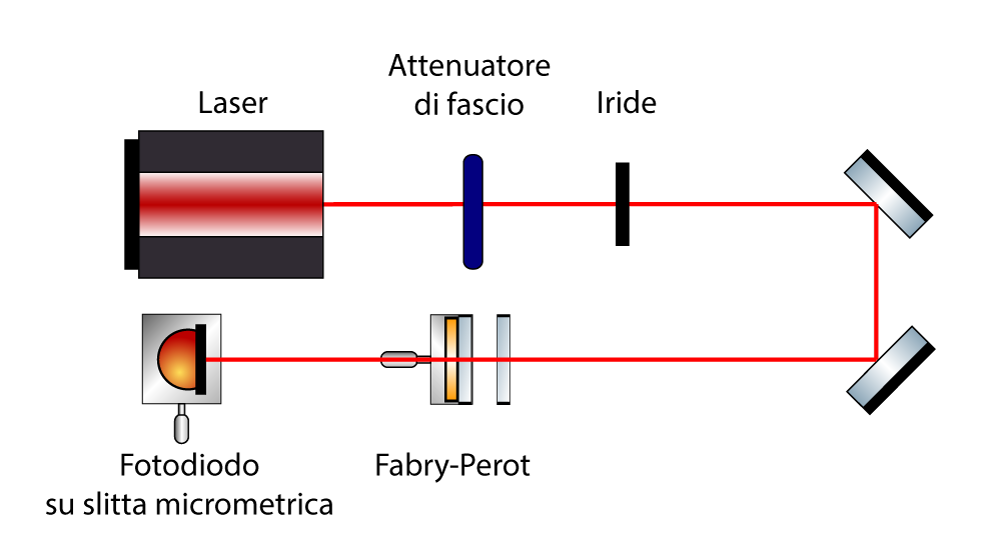
\includegraphics[width=1.1\linewidth]{diagram.png}}
	\captionof{figure}{Configurazione utilizzata.}
	\label{fig:diagram}
	\end{center}
\end{Figure}

Il segnale in uscita dal fotodiodo è inviato al \texttt{CH 2} dell'oscilloscopio \texttt{Tektronik TDS2012C}. Le misure di intensità luminosa vengono riportate come differenza di potenziale misurata ai capi del fotodiodo, pertanto è da intendere la presenza di un fattore di proporzionalità non noto. Inoltre, si regola con un filtro attenuatore l'intensità della luce emessa dal laser in modo da restare all'interno della regione di linearità del fotodiodo, ossia al di sotto di \SI{10}{V}. L'incertezza associata alle misure mediante i cursori è quella fornita dal manuale\footnote{\url{http://pdf1.alldatasheet.com/datasheet-pdf/view/554089/ETC2/TDS2012C.html}} dell'oscilloscopio, ossia il $3\%$.

Poiché il fotodiodo permette l'ingresso della luce attraverso un foro di diametro circa \SI{200}{\micro m}, si compiranno spostamenti della slitta micrometrica di almeno \SI{100}{\micro m}, e pertanto l'incertezza associata alla posizione del fotodiodo sarà di \SI{100}{\micro m}.

%==================================================
%             FIT DELLA FUNZIONE DI AIRY
%==================================================
\section{Misura della funzione di trasmissione e fit alla funzione di Airy}
In questa parte dell'esperienza si utilizzano specchi di riflettività $R=0.9$. Dalla relazione 
\begin{equation}\label{eq:finesse}
F_{teo} = \frac{\pi\sqrt R}{1-R}
\end{equation}
si ricava un valore teorico di finesse $F_{teo} = 29.8$. La ceramica piezoelettrica montata sulla slitta viene pilotata da un segnale triangolare, al fine di osservare due massimi della funzione di trasmissione. Si imposta il filtro attenuatore in modo da avere intensità massima $I_{max} = \SI{6.4\pm0.2}{V}$, ben al di sotto della regione di saturazione. Si acquisiscono i punti sperimentali relativi al segnale di rampa e alla risposta del fotodiodo, in funzione del tempo\footnote{Si prende l'origine temporale $t=0$ coincidente con l'istante in cui viene effettuata la prima misura.}, direttamente dall'oscilloscopio, e si riportano tali punti nel grafico di Figura~\ref{fig:fit-airy}.

Si effettua il fit dei dati sperimentali usando come espressione per la funzione di Airy \begin{equation}\label{eqn:airy}
T=\frac{1}{1+\frac{4F_{exp}^2}{\pi^2}\,\sin^2\big(A(V_{tr}-V_0)\big)},
\end{equation}
espressa in funzione della finesse sperimentale $F_{exp}$ e dello sfasamento $\Delta/2 = A(V_{\text{tr}}-V_0)$, dove $V_{\text{tr}}$ è il valore della tensione dell'onda triangolare, e normalizzata al massimo dell'intensità. Sono stati introdotti i parametri $A$ e $V_0$ rappresentanti rispettivamente il coefficiente di proporzionalità tra lo sfasamento e la tensione dell'onda triangolare, ed il fattore traslazione della funzione di trasferimento lungo l'asse delle ascisse. 

Il fit, riportato in Figura (\ref{fig:fit-airy}), ha come coefficienti 
\begin{align*}
&F_{exp} = \SI{29.1\pm0.9}{}\\[0.2cm]
&A = \SI{0.472\pm0.002}{V^{-1}}\\[0.2cm]
&V_0 = \SI{3.01\pm0.02}{V}
\end{align*}
Il valore sperimentale di finesse risulta compatibile, entro una deviazione standard, con quello teorico. 

\begin{Figure}
	\begin{center}
	\hbox{\hspace{-0.8cm}
	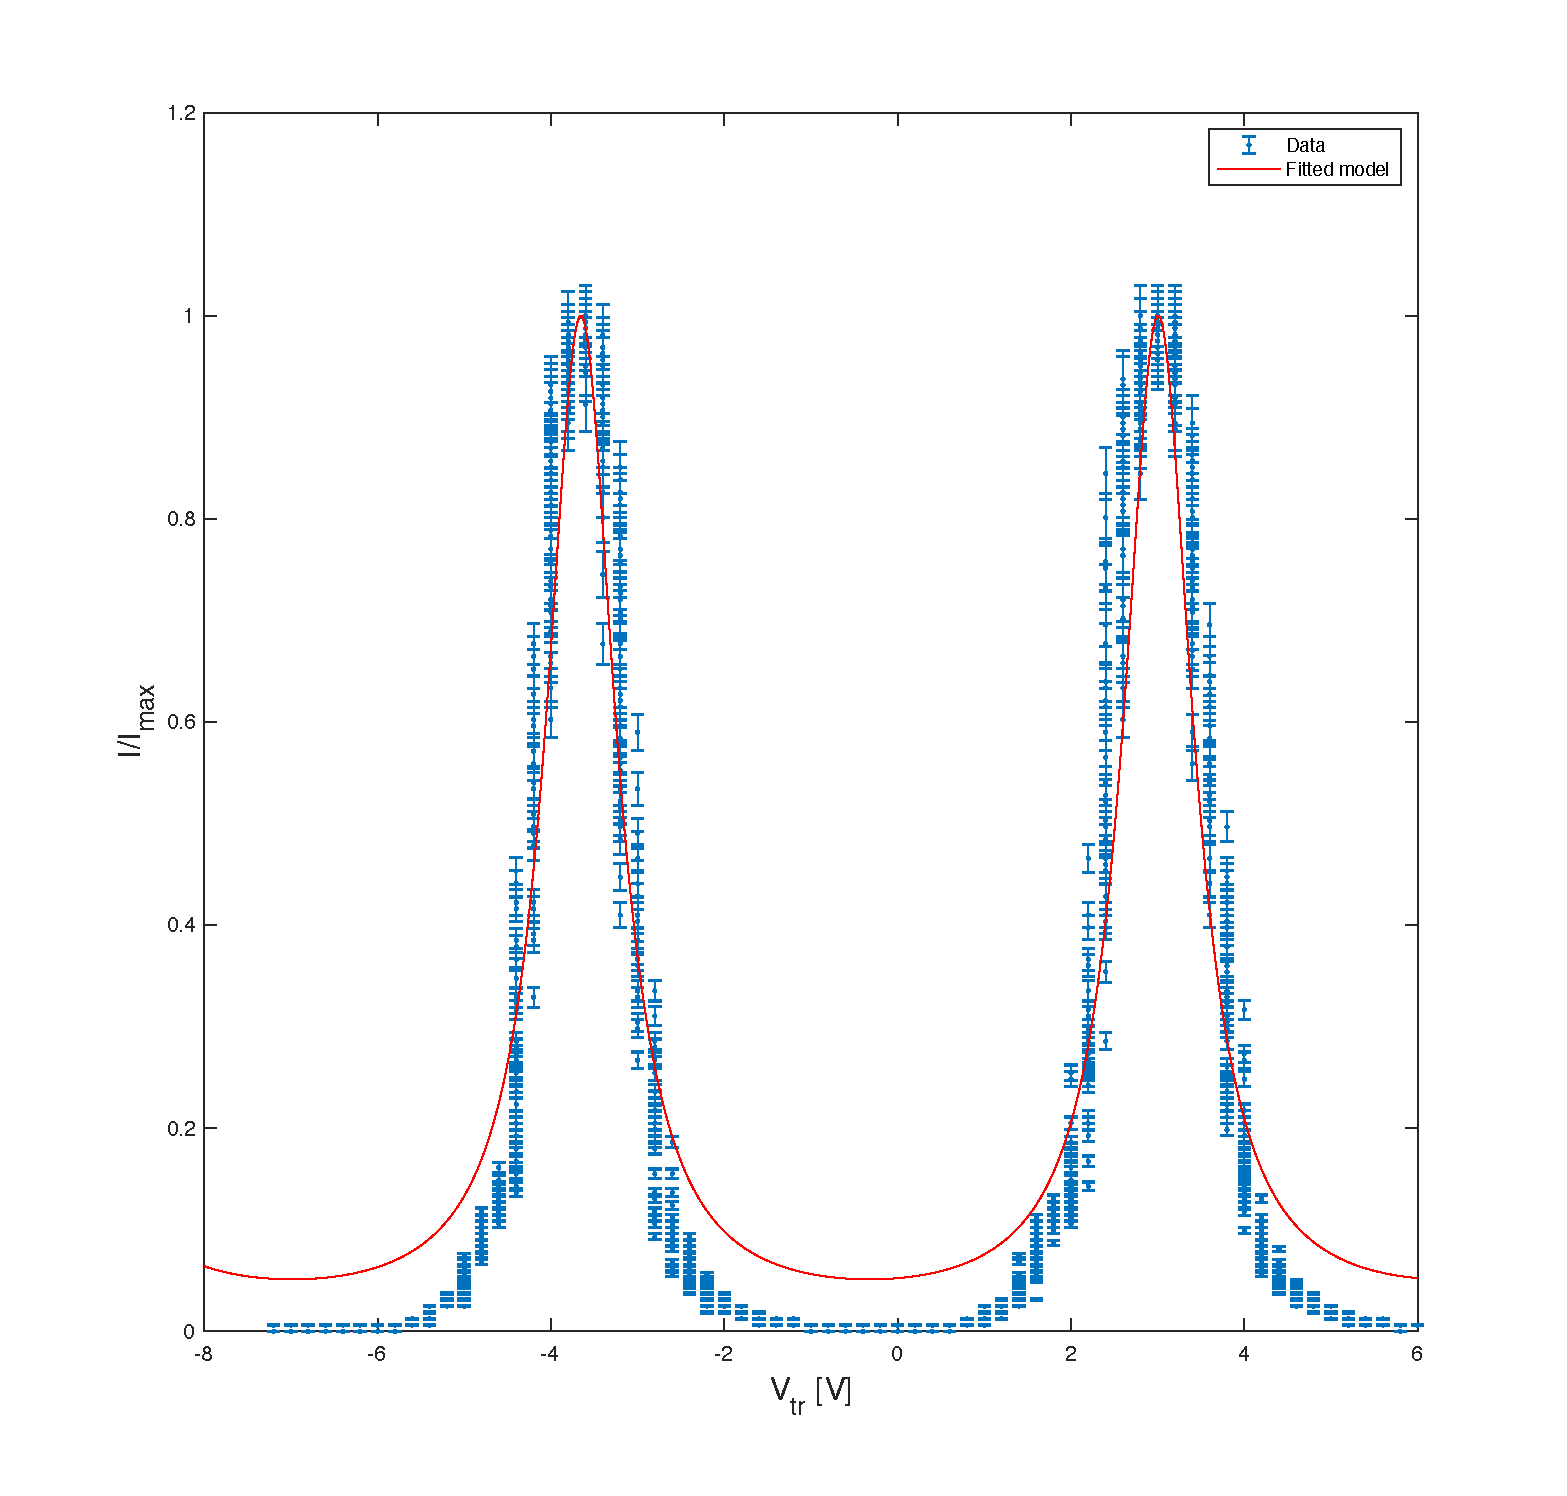
\includegraphics[width=1.1\linewidth]{fit-airy}}
	\captionof{figure}{Fit della funzione di Airy.}
	\label{fig:fit-airy}
	\end{center}
\end{Figure}

Si ricorda che $\Delta = b\,V_{tr}$ con \[
b = \frac{2\pi}{V_{tr_N}-V_{tr_{N+1}}},
\]
dove $V_{tr_N}$ è il valore di tensione dell'onda triangolare corrispondente al picco di ordine $N$. Il valore del parametro $A$ è dunque da confrontarsi con \[
\frac{b}{2} = \SI{0.476\pm0.001}{V^{-1}},
\]
che risulta essere compatibile, entro due sigma, con il valore ricavato dal fit.

Si osserva come la curva di fit sia più vicina a quella sperimentale in corrispondenza dei massimi, mentre è evidente come i minimi delle due siano molto più distanti, al di fuori delle barre di incertezza. Si ritiene che questo sia dovuto alla ridotta sensibilità del fotodiodo nella regione in cui il segnale è comparabile con il fondo, che non permette di discriminare tra i due; oltretutto, si ipotizza che in prossimità dei minimi non sia superata la tensione di soglia del rivelatore, al di sotto della quale non vi è linearità della risposta. L'identificazione della larghezza dei massimi e della distanza tra essi è però indipendente dall'andamento della tensione nella regione compresa tra essi, e pertanto non compromette la qualità della stima della \emph{finesse}.  


%==================================================
%             MISURA DELLA FINESSE
%==================================================
\section{Misura della finesse al variare delle combinazioni di specchi}
Nella relazione~(\ref{eq:finesse}) per la \emph{finesse} $\mathcal{F}$ si utilizzerà come valore di $R$ la media geometrica delle riflettività dei due specchi utilizzati per costruire l'interferometro. Assumendo che la dilatazione della ceramica sia lineare rispetto alla tensione $V_\text{tr}$ applicata, si deduce che la variazione di fase $\Delta$ tra le onde piane uscenti dall'interferometro, proporzionale alla variazione di distanza $D$ tra i due specchi dell'interferometro, è anch'essa lineare in $V_\text{tr}$, cioè si assume che
\[
	\Delta = b V_\text{tr}.
\]
Per stimare il coefficiente di proporzionalità $b$ si prendono le misure $V$ e $\tilde{V}$ di tensione corrispondenti a due massimi consecutivi che siano sulla stessa rampa dell'onda triangolare, uguagliando le intensità corrispondenti ai due diversi ordini si trova che
\begin{equation}\label{eq:b}
	b=\frac{2\pi}{\tilde{V}-V}.
\end{equation}

Inoltre, nell'approssimazione in cui ${\Delta V b/ 2 \ll 1}$, si stima la larghezza a metà altezza $\Delta V$ del picco della funzione di Airy imponendo che l'intensità sia pari a metà di quella massima, e si trova
\begin{equation}\label{eq:F_approx}
	\mathcal{F} \simeq \frac{\tilde{V} - V}{2 \Delta V}.
\end{equation}

Poiché si utilizza un segnale triangolare si ha proporzionalità tra la tensione della rampa e l'istante di tempo a cui sono riferiti i punti sperimentali, rispetto ad uno zero arbitrario. Le misure di tensione vengono pertanto sostituite con misure di tempo, più convenienti poiché sono riportate sull'ascissa dell'oscilloscopio, effettuate mediante i cursori dello strumento. Si determinano pertanto la distanza temporale tra due picchi e la larghezza a metà altezza degli stessi.
 
Si ripetono tali misure per diverse combinazioni di specchi; esse sono riportate in Tabella \ref{tab:parte_due}, in Appendice. Si riportano in Figura \ref{fig:parte_due_retta} i valori di $\mathcal{F}^{-2}$ ricavati sperimentalmente, con $\mathcal{F}$ stimata da (\ref{eq:F_approx}), in funzione di $F_\mathrm{teo}^{-2}$, dove $F_\mathrm{teo}$ è la finesse teorica data da (\ref{eq:finesse}).
\begin{Figure}
	\begin{center}
	\hbox{\hspace{-0.8cm}
	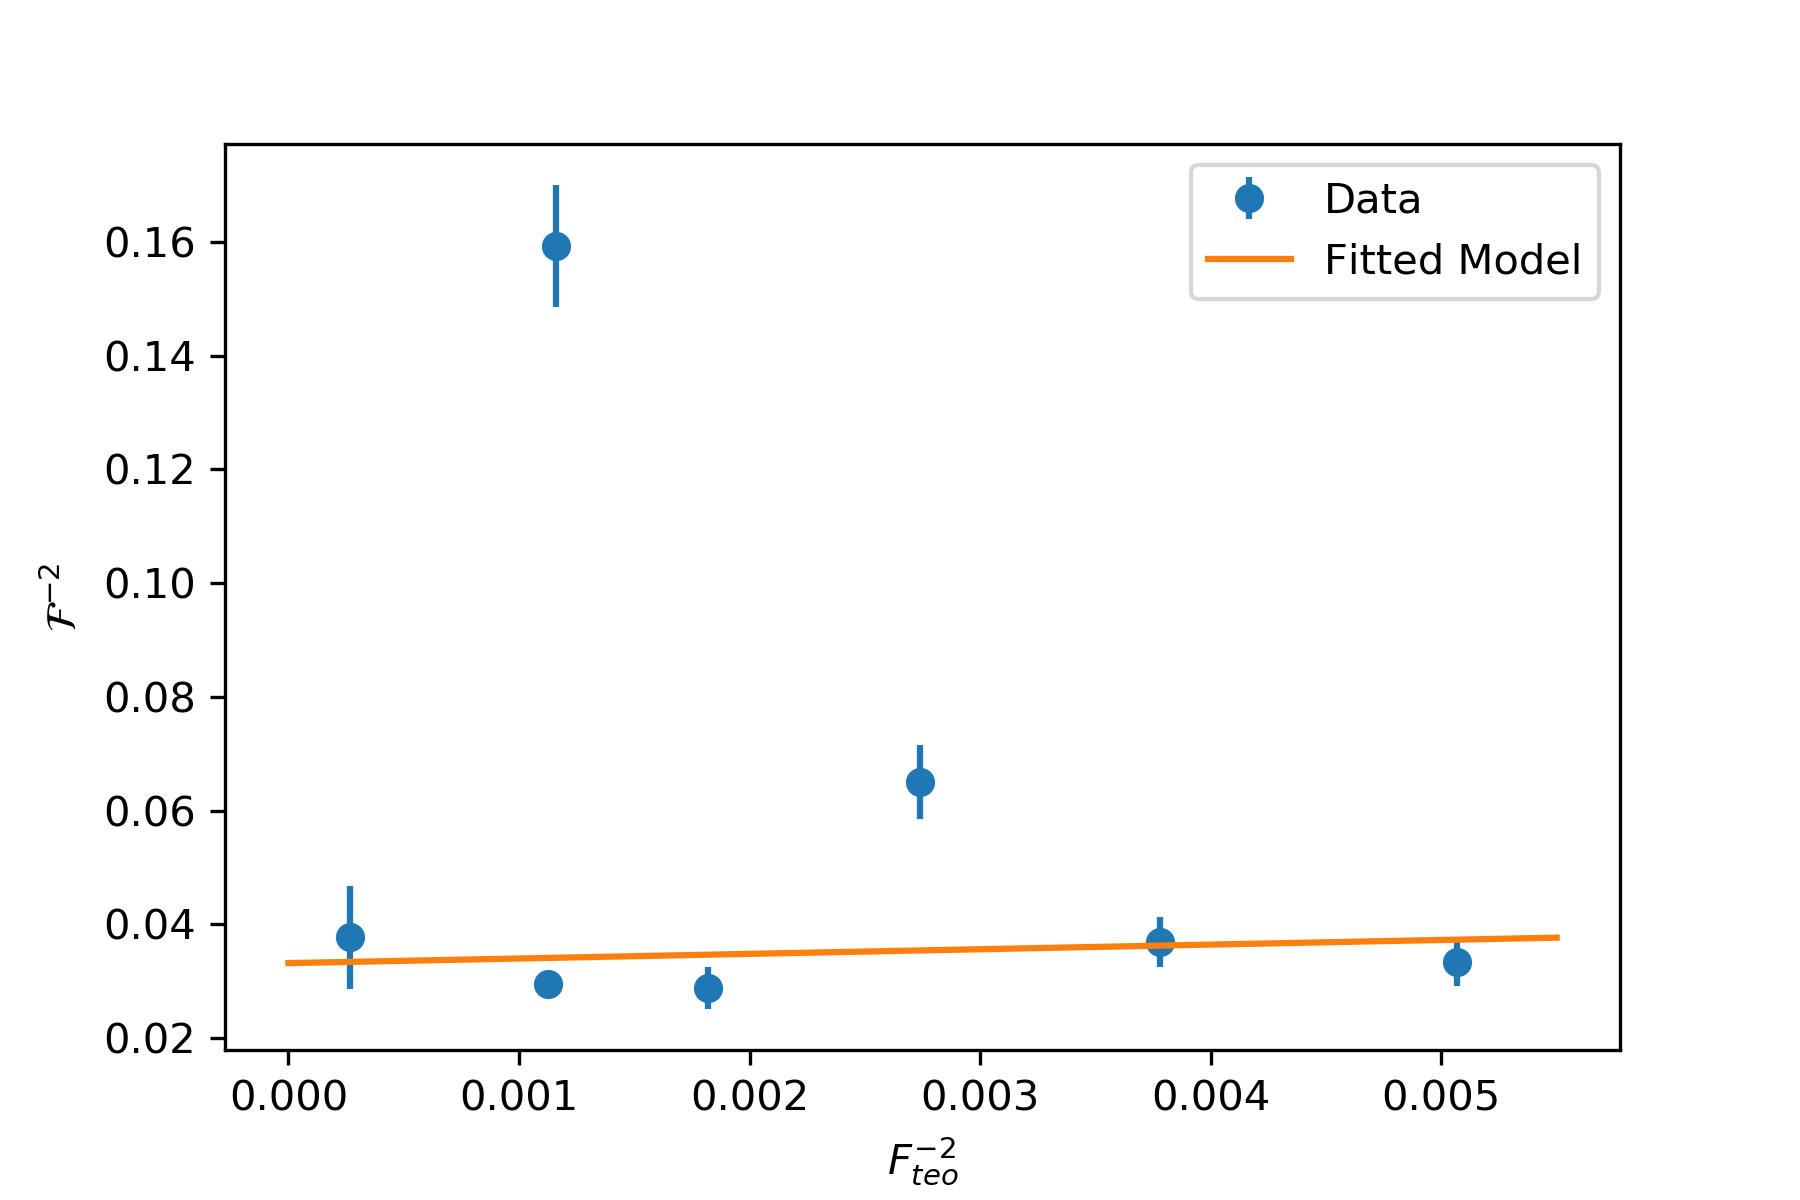
\includegraphics[width=1.1\linewidth]{parte_due_fit.png}}
	\captionof{figure}{Andamento del quadrato del reciproco della finesse sperimentale in funzione del quadrato del reciproco della finesse ideale}
	\label{fig:parte_due_retta}
	\end{center}
\end{Figure}

Come è evidente, le misure si discostano molto dall'andamento previsto: ci si aspettava infatti un andamento lineare con coefficiente angolare unitario e intercetta positiva. Al contrario, il coefficiente angolare restituito dal fit risulta essere $0.8$, ma con chi quadro di ordine \SI{1.6 e4}{}, che caratterizza la scarsa aderenza al modello teorico. Si conclude che questo sia dovuto ad un errore sistematico nell'allineamento del sistema: l'allineamento è stato infatti realizzato sistematicamente al fine di massimizzare la visibilità delle frange, ma non si è verificato ad ogni cambiamento di specchi che il centro della figura di interferenza fosse allineato con il fotodiodo. D'altra parte, infatti, una ulteriore misura fatta allineando correttamente il sistema ha restituito per la finesse il valore di \SI{9.1 \pm 0.9}{} contro un valore teorico previsto di $14$ ($R=0.8$), meno discosto dalla teoria rispetto agli altri punti.

%==================================================
%             MISURA DI LAMBDA
%==================================================
\section{Misura della lunghezza del Fabry-Perot e stima della lunghezza d'onda del laser}
Si verifica che per tutta la durata di questa presa dati il voltaggio del fotodiodo rimane compreso tra \SI{0}{} e \SI{0.6}{V}, dunque nella regione di linearità. Si rammenta che la distanza tra il fotodiodo e il secondo specchio del Fabry-Perot è $L=\SI{209 \pm 2}{mm}$; si interpone dunque tra il secondo specchio metallico e l'interferometro un foglio di plastica trasparente opaco quale mezzo diffusore, al fine di ottenere un'onda analoga a quella generata da una sorgente puntiforme. Oltre l'interferometro si osserva dunque il pattern di massimi e minimi circolari detto \emph{anelli di Airy}.

Si verifica che la posizione assoluta del secondo specchio dell'interferometro, rispetto allo zero della vite micrometrica che non necessariamente corrisponde alla distanza nulla tra gli specchi, è $d_1 = \SI{13.37 \pm 0.01}{mm}$.

Traslando la slitta su cui è posto il fotodiodo si misurano le posizioni di due massimi consecutivi e se ne stima l'angolo rispetto al centro del pattern come $\theta = (x-x_0) / L$. Si ha la relazione tra ordine del massimo e angolo 
\begin{equation}\label{eq:diff}
\frac{2d^f}{\lambda} \cos{\theta_m} = m
\end{equation}
sviluppando il coseno al secondo ordine si ottiene, dalla misura di due angoli,
\[
m \simeq \frac{2}{\theta_{m-1}^2 - \theta_{m}^2}
\]
e conoscendo il valore della lunghezza d'onda $\lambda$ (come dichiarato dal costruttore) si ottiene una stima della lunghezza del Fabry-Perot
\[
d^f \simeq \frac{m \lambda}{2},
\]
valida per $m \gg 1$.

Variando quindi la posizione assoluta del secondo specchio del Fabry-Perot, e portandolo a $d_2 = \SI{10.75 \pm 0.01}{mm}$, si ripete il procedimento precedente e si ricava l'ordine del massimo $m_2$. Quindi, si può stimare la lunghezza d'onda del laser da \[
\lambda^{\text{exp}} = \frac{2(d_1 - d_2)}{m_2 - m_1}.
\]

Si riportano in Tabella~\ref{tab:stimaLambda}, in Appendice, i dati raccolti. La stima della lunghezza d'onda risulta essere
\[
\lambda^{\text{exp}} = \SI{ 181 \pm 46}{nm},
\]

e le corrispondenti lunghezze $d_i^f$ del Fabry-Perot

\[
\begin{aligned}
d_1^f &= \SI{2.8 \pm 0.9}{mm} \\
d_2^f &= \SI{0.21 \pm 0.07}{mm}
\end{aligned}
\]

Il termine dominante nel calcolo delle incertezze risulta essere quello relativo all'ordine di diffrazione. Osserviamo che il valore di $\lambda$ determinato sperimentalmente non è compatibile con quello dichiarato dal costruttore. Nemmeno le lunghezze del Fabry Perot sono coerenti con quanto osservato durante l'esperimento, dove l'ordine di grandezza della separazione degli specchi è di circa \SI{1}{cm}. Consideriamo i dati raccolti quando lo specchio mobile dell'interferometro si trova a una distsanza assoluta $d_2$. Secondo la relazione~(\ref{eq:diff}) all'aumentare di $m$ la distanza relativa tra due massimi consecutivi dovrebbe ridursi per via della funzione coseno. Questo non accade nei dati sperimentali raccolti, dove $x_1-x_0 < x_2-x_1$. Ciò porta a pensare a errori di lettura nella presa dati, in particolare di $x_2$, a causa di un non corretto allineamento del fascio. Si ritiene infatti che il fotodiodo non abbia rilevato correttamente la presenza di un massimo intermedio, in quanto non avente intensità sufficientemente superiore a quella di soglia.
Utilizzando invece la lunghezza d'onda fornita dal costruttore $\lambda = \SI{632.8}{nm}$ e gli ordini ricavati $m_1$ e $m_2$ si ottiene rispettivamente
\[
\begin{aligned}
d_1^f &= \SI{1 \pm 0.2}{cm} \\
d_2^f &= \SI{0.73 \pm 0.03}{mm}
\end{aligned}
\]

Osserviamo che $d_1^f-d_2^f$ non è compatibile con $d_1 - d_2$. Ciò rafforza l'ipotesi di errori nella stima dell'ordine di diffrazione per la seconda configurazione. Tuttavia, limitandosi alla prima presa dati, si ritiene che la stima della lunghezza del Fabry-Perot sia compatibile con la reale distanza tra gli specchi, che risultava essere, misurata con il metro a nastro, \SI{1.2 \pm 0.2}{cm}.



%==================================================
%             CONCLUSIONI
%==================================================
\section{Conclusioni}
Dal fit della funzione di trasmissione con la funzione di Airy si ricava un valore della finesse compatibile con quello teorico. Si è infatti allineato, prima della presa dati, il centro del pattern circolare con il foro del fotodiodo. Al contrario, nella seconda parte, non si è prestata altrettanta attenzione all'allineamento del pattern, ritenendo che la lettura su una frangia vicina potesse portare allo stesso risultato. Si sarebbe potuto adoperare il mezzo diffusore al fine di visualizzare l'intera figura e agevolare l'allineamento.

Si osserva inoltre come la non compatibilità dei punti sperimentali rispetto al modello teorico sia dovuta alla non idealità concettuale dell'apparato: gli specchi non sono infatti perfettamente piani e presentano delle rugosità e imperfezioni, l'onda incidente non è piana (l'andamento è meglio descritto da un fascio gaussiano) e l'allineamento inficia la accuratezza delle misure.

Infine, nella terza parte si ritiene che la scelta di specchi ad elevata riflettività ($R=0.9$) abbia influito sulla lettura dell'intensità da parte del fotodiodo, e sulla conseguente identificazione dell'ordine di interferenza, in quanto è stata ridotta notevolmente l'intensità del fascio.

\end{multicols}


\newpage
\section{Appendice}

\begin{center}
\captionof{table}{Misure per la stima di $\lambda$}
\label{tab:stimaLambda}
\begin{tabular}{c|c|c|c|c|c}
 & $x_0$ [\SI{}{mm}] & $x_1$ [\SI{}{mm}] & $x_2$ [\SI{}{mm}] & $\theta_1$  & $\theta_2$ \\
 & $\pm 0.01$ & $\pm 0.1$ & $\pm 0.1$ & & \\
\hline 
$d_1 = \SI{13.37 \pm 0.01}{mm}$ & 10.70  & 12.7 & 11.8 &    \SI{9.6 \pm 0.7 e-3}{} & \SI{5.3 \pm 1.0 e-3}{} \\
$d_2 = \SI{10.75 \pm 0.01}{mm}$ & 14.80   & 13.1 & 8.4  & \SI{8.1 \pm 0.7 e-3}{} & \SI{31.0 \pm 0.7 e-3}{} \\
\hline
\end{tabular}
\newline
\vspace*{0.4cm}
\newline
\begin{tabular}{c|c|c|c}
& m & $d^f [\SI{}{mm}]$ & $d^f [\SI{}{mm}]$, $\lambda=\SI{632.8}{nm}$ \\
\hline
$d_1 = \SI{13.37 \pm 0.01}{mm}$ & \SI{31 \pm 7 e3}{} & \SI{2.8 \pm 0.9}{} & \SI{10 \pm 2}{}\\
$d_2 = \SI{10.75 \pm 0.01}{mm}$ & \SI{2.3 \pm 0.1 e3}{}  & \SI{0.21 \pm 0.07}{} & \SI{0.73 \pm 0.03}{}\\
\hline
\end{tabular}
\end{center}


\begin{center}
\captionof{table}{Misure per la stima di $\mathcal F$.}
\label{tab:parte_due}
\begin{tabular}{c|c|c|c|c}
$R_1$ & $R_2$ & $V$ [\SI{}{ms}] & $\tilde V$ [\SI{}{ms}] & $2\Delta V$ [\SI{}{ms}]\\
\hline
 0.90 & 0.90 &  14 $\pm$ 2 & 427 $\pm$  2 &  71 $\pm$  3 \\
 0.95 & 0.95 & 196 $\pm$ 8 & 608 $\pm$ 8 &  80  $\pm$11 \\
 0.90 & 0.80 &  84 $\pm$ 4 & 476 $\pm$  4 & 100$\pm$   6 \\
 0.90 & 0.85 & 532 $\pm$ 4 & 968 $\pm$ 4 &  74  $\pm$ 6 \\
 0.80 & 0.85 & 340 $\pm$ 4 & 756 $\pm$ 4 &  80  $\pm$ 6 \\
 0.95 & 0.85 & 324 $\pm$ 4 & 740 $\pm$ 4 & 166 $\pm$  6 \\
 0.80 & 0.80 & 332 $\pm$ 4 & 748 $\pm$ 4 &  76  $\pm$ 6 \\
\hline
\end{tabular}
\end{center}











%ESEMPIO DI FIGURA
%\begin{Figure}
%	\begin{center}
%	\includegraphics[width=\linewidth]{comune.png}
%	\captionof{figure}{Istantanea dell'oscilloscopio per l'amplificatore differenziale, misura di $A_c$}
%	\label{fig:Ac_differenziale}
%	\end{center}
%\end{Figure}


%ESEMPIO DI TABELLA
%\begin{center}
%\captionof{table}{Misure per la stima di $A_c$}
%\label{tab:Ac_differenziale}
%\begin{tabular}{c|c|c|c}
%$f$ [\SI{}{Hz}] & $V_i$ [\SI{}{V}] & $v_o$ [\SI{}{mV}] & $A_c = v_o / V_i$ \\
%\hline
%      149.5 &        3.90 &         11.3 & 2.90e-03 \\
%      222.0 &        3.90 &         11.5 & 2.95e-03 \\
%      281.0 &        3.90 &         11.8 & 3.03e-03 \\
%      359.0 &        3.90 &         11.8 & 3.03e-03 \\
%      461.0 &        3.90 &         12.2 & 3.13e-03 \\
%\hline
%\end{tabular}
%\end{center}

\end{document}
